% Template for PLoS
% Version 3.5 March 2018
%
% % % % % % % % % % % % % % % % % % % % % %
\documentclass[10pt,letterpaper]{article}
\usepackage[top=0.85in,left=2.75in,footskip=0.75in]{geometry}
% FIGURES
\usepackage{graphicx}
\usepackage{pgf}
% amsmath and amssymb packages, useful for mathematical formulas and symbols
\usepackage{amsmath,amssymb}
% Use adjustwidth environment to exceed column width (see example table in text)
\usepackage{changepage}
% Use Unicode characters when possible
\usepackage[utf8x]{inputenc}
% textcomp package and marvosym package for additional characters
\usepackage{textcomp,marvosym}
% cite package, to clean up citations in the main text. Do not remove.
\usepackage{cite}
% Use nameref to cite supporting information files (see Supporting Information section for more info)
\usepackage{nameref,hyperref}
% line numbers
\usepackage[right]{lineno}
% ligatures disabled
\usepackage{microtype}
\DisableLigatures[f]{encoding = *, family = * }
% color can be used to apply background shading to table cells only
\usepackage[]{xcolor}
% array package and thick rules for tables
\usepackage{array}
% create "+" rule type for thick vertical lines
\newcolumntype{+}{!{\vrule width 2pt}}
% create \thickcline for thick horizontal lines of variable length
\newlength\savedwidth
\newcommand\thickcline[1]{%
  \noalign{\global\savedwidth\arrayrulewidth\global\arrayrulewidth 2pt}%
  \cline{#1}%
  \noalign{\vskip\arrayrulewidth}%
  \noalign{\global\arrayrulewidth\savedwidth}%
}
% \thickhline command for thick horizontal lines that span the table
\newcommand\thickhline{\noalign{\global\savedwidth\arrayrulewidth\global\arrayrulewidth 2pt}%
\hline
\noalign{\global\arrayrulewidth\savedwidth}}
% Text layout
\raggedright
\setlength{\parindent}{0.5cm}
\textwidth 5.25in 
\textheight 8.75in
% Bold the 'Figure #' in the caption and separate it from the title/caption with a period
% Captions will be left justified
\usepackage[aboveskip=1pt,labelfont=bf,labelsep=period,justification=raggedright,singlelinecheck=off]{caption}
\renewcommand{\figurename}{Fig}
% Remove brackets from numbering in List of References
\makeatletter
\renewcommand{\@biblabel}[1]{\quad#1.}
\makeatother
% Header and Footer with logo
\usepackage{lastpage,fancyhdr,graphicx}
\usepackage{epstopdf}
\pagestyle{fancy}
\fancyhf{}
\rfoot{\thepage/\pageref{LastPage}}
\renewcommand{\headrulewidth}{0pt}
\renewcommand{\footrule}{\hrule height 2pt \vspace{2mm}}
\fancyheadoffset[L]{2.25in}
\fancyfootoffset[L]{2.25in}
\lfoot{\today}
%% Include all macros below
\newcommand{\lorem}{{\bf LOREM}}
\newcommand{\ipsum}{{\bf IPSUM}}
%% END MACROS SECTION
%%%%%%%%%%%%%%%%%%%%%%%%%%%%%%%%%%%%%%%%%%%%%%%%%%%%%%%%%%%%%%%%%%%%%%%%%%%%%%%%%%%%%%%%%%


\begin{document}
\vspace*{0.2in}

% TITLE
\begin{flushleft}
{\Large
\textbf\newline{
Analysis of heatwaves in UKCP18 climate projections
}}
\newline
\\
Kevin Donkers\textsuperscript{1,2*}
\\
\bigskip
\textbf{1} Environmental Intelligence CDT, University of Exeter, Exeter, Devon, UK
\\
\textbf{2} Informatics Lab, Met Office, Exeter, Devon, UK
\\
\bigskip
* kevin.donkers@informaticslab.co.uk
\end{flushleft}


% ABSTRACT (below 300 words)
\section*{Abstract}

As global average temperatures continue to increase under climate change, extreme events will become more common and previously impossible events the new extremes. The impacts of high temperatures are far reaching and the increased likelihood of extreme heatwaves is already being felt, for instance with the 2003 European heatwave which caused about 70,000 excess deaths\cite{Vautard2020}. In the UK the Met Office define a heatwave as three or more consecutive days of daily maximum temperatures exceeding a given threshold temperature, as defined by the local climatology.\cite{McCarthy2019} We use this to analyse the number and duration of heatwaves projected to occur in London under the UKCP18 climate projections. In addition we conduct this heatwave analysis using a Universal Thermal Climate Index (UTCI) adjustment to the maximum daily air temperature, which factors in humidity and windspeed to provide a more physiologically accurate representation of high temperatures. This could be used to overcome some of the assumptions posed in the Met Office heatwave definition in order to define a more universal heatwave definition.

% INTRODUCTION
\section*{Introduction}

As global mean temperatures increase due to climate change, heatwaves are expected to get hotter, longer and more frequent. 
Indeed we are already seeing many more unprecedented heatwaves in Europe, starting in 2003 with the hottest heatwave for 500 years\cite{Stott2004} and continuing to break records in 2019, the latter being statistically attributed to anthropogenic climate change.\cite{Vautard2020} 
The UK heatwave in August 2020 was another record breaker.\cite{Askew2020}
Heatwaves in the UK have been shown to increase human morbidity\cite{Smith2016}, mortality\cite{Johnson2004} and disruption to critical infrastructure.\cite{Dawson2016}


The Met Office Hadley Centre has been working on climate change predictions since the early 1990s.
The Centre has developed and published data from a series of global climate models called HadGEM.
These models are used to initiate a series of regional climate models, HadREM, which produce climate predictions on a finer spatial resolution.
About every decade a regional climate model is run and published for the UK.
The latest of these, UKCP18, provides data on a range of spatial scales and emissions scenarios.\cite{UKCP18}
These include convection permitting models (CPM) which go down to a 2.2 km spatial resolution and can start to resolve convective weather, an important feature with regards to predicting intense precipitation events.
All meteorological variables in this model output are available at a daily temporal resolution, with air temperature available up to hourly.
This means that UKCP18 data can be used to predict heatwave activity in the UK for the rest of the 21\textsuperscript{st} century.

\pagebreak
\noindent
The World Meteorological Organisation defines a heatwave as:
\begin{quote}
    A period of marked unusual hot weather over a region persisting for at least three consecutive days during the warm period of the year based on local climatological conditions, with thermal conditions recorded above given thresholds.\cite{WMO2018}
\end{quote}
The UK Met Office uses this definition to specify a heatwave as three or more consecutive days where the maximum daily air temperature exceeds a threshold defined by the local climatology, as published by McCarthy \textit{et al.}.\cite{McCarthy2019}
In this case the threshold is the 90{\textsuperscript{th}} percentile of maximum daily temperature within a county for July in years 1981-2010, rounded to nearest whole °C.
This definition was chosen for both its correlation with public perception that a heatwave is an uncommon event and the need for national meteorological services to issue warnings infrequently enough so as not to lose their efficacy.
To these ends, the definition achieves its aims.
However, a number of critiques can be raised about this definition.

First, the baseline period that this definition uses is well within living memory but also includes a number of the ten hottest years on record.\cite{McCarthy2019}
This is good in terms of public perception but bad for comparing heatwave events decades in the future as heatwave events are expected to increase in frequency and the future public is likely to perceive a different baseline.

Second, McCarthy \textit{et al.} define the threshold on a county by county basis, which is convenient for public communication but not universal or applicable to all areas of a county.
For instance, many coastal counties in England experience the full range of 90\textsuperscript{th} percentile July maximum daily temperatures used to define the threshold, as seen in Fig ~\ref{McCarthy-fig3}.\cite{McCarthy2019}
Similarly, urban areas which experience greater overall temperatures than the surrounding rural areas of the same county, due to urban heat island effects, will have a less relevant threshold if the rural areas make up the majority of the county land area.

Third, air temperature may be a good indicator of how hot conditions feel, but physiologically accurate estimates of heat stress rely on multiple meteorological factors, such as humidity and wind speed, and non-meteorological factors, such as the temperature of physical surroundings and availability of shading.
Basing a heatwave definition on maximum daily temperature alone is simple and broadly representative of the meteorological conditions that tend to accompany heat waves the UK (summer high-pressure systems), but this may not always be the case as the UK's climate heats up and unprecedented weather patterns emerge.

Therefore, an alternative to basing heatwave definitions on maximum daily air temperature and a local threshold would be to base them on biometeorological heat stress metrics which factor in human physiological responses to high temperatures.
This would allow heatwaves to be defined in terms of their effects on people rather than a perceived unusuality of events.
Over 100 such metrics have been defined in the literature, but Universal Thermal Climate Index (UTCI) was found to be most suitable at representing human response to thermal stress under a variety of climatic and meteorological conditions.\cite{Blazejczyk2012, DiNapoli2018, Zare2018}
Błażejczyk, one of the originators of UTCI, defines it as:
\begin{quote}
    The air temperature ($T_a$) of the reference condition causing the same model response as actual conditions.\cite{Blazejczyk2012}
\end{quote}
Essentially, UTCI is the temperature in the reference conditions that would elicit exactly the same physiological response as the real-world conditions being considered.

\pagebreak
\noindent
This reference condition is defined as:
\begin{itemize}
    \item Relative humidity ($RH$) of $50\%$
    \item Wind speed ($v_w$) of $0.5 ms^{-1}$ at $10 m$ or $0.3 ms^{-1}$ at $1.5 m$
    \item Mean radiant temperature ($T_{mrt}$) equal to the air temperature (i.e. physical surrounds in thermal equilibrium with the air)
\end{itemize}
Mathematically the relationship can be represented by:
\begin{align*}
    UTCI &= f(T_a, T_{mrt}, RH, v_w) \\
    &= T_a + \text{Offset}(T_a, T_{mrt}, RH, v_w)
\end{align*}
The offset can be approximated by a 6\textsuperscript{th} order polynomial of $T_a$, $T_{mrt}-T_a$, $RH$ and $v_w$.\cite{Blazejczyk2013}
UTCI values can be banded into ten categories with specific physiological responses to thermal stress, as seen in Table~\ref{utci-table}.

\begin{table}[]
\centering
\caption{
{\bf UTCI thermal stress categories.\cite{Blazejczyk2013}}}
\begin{tabular}{|l|l|}
\hline
\textbf{UTCI (°C) range} & \textbf{Thermal stress category} \\ \thickhline
greater than 48 & Extreme heat stress     \\ \hline
38 to 48        & Very strong heat stress \\ \hline
32 to 38        & Strong heat stress      \\ \hline
26 to 32        & Moderate heat stress    \\ \hline
9 to 26         & No thermal stress       \\ \hline
0 to 9          & Slight cold stress      \\ \hline
0 to -13        & Moderate cold stress    \\ \hline
-13 to -27      & Strong cold stress      \\ \hline
-27 to -40      & Very strong cold stress \\ \hline
less than -40   & Extreme cold stress     \\ \hline
\end{tabular}
\label{utci-table}
\end{table}


The purpose of this project is, therefore, to compare the number and duration of heatwave events in the UKCP18 climate change for the three decades available (1981-2000, 2021-2040 and 2061-2080), using the Met Office heatwave definition, the UTCI heat stress definition and a combination of UTCI values with local climatology threshold.
Due to computer processing constraints, all the analysis in this project was conducted on a spatial subset of the data representing the Greater London area.

\begin{figure}
% \begin{adjustwidth}{-2.25in}{0in}
    \begin{center}
        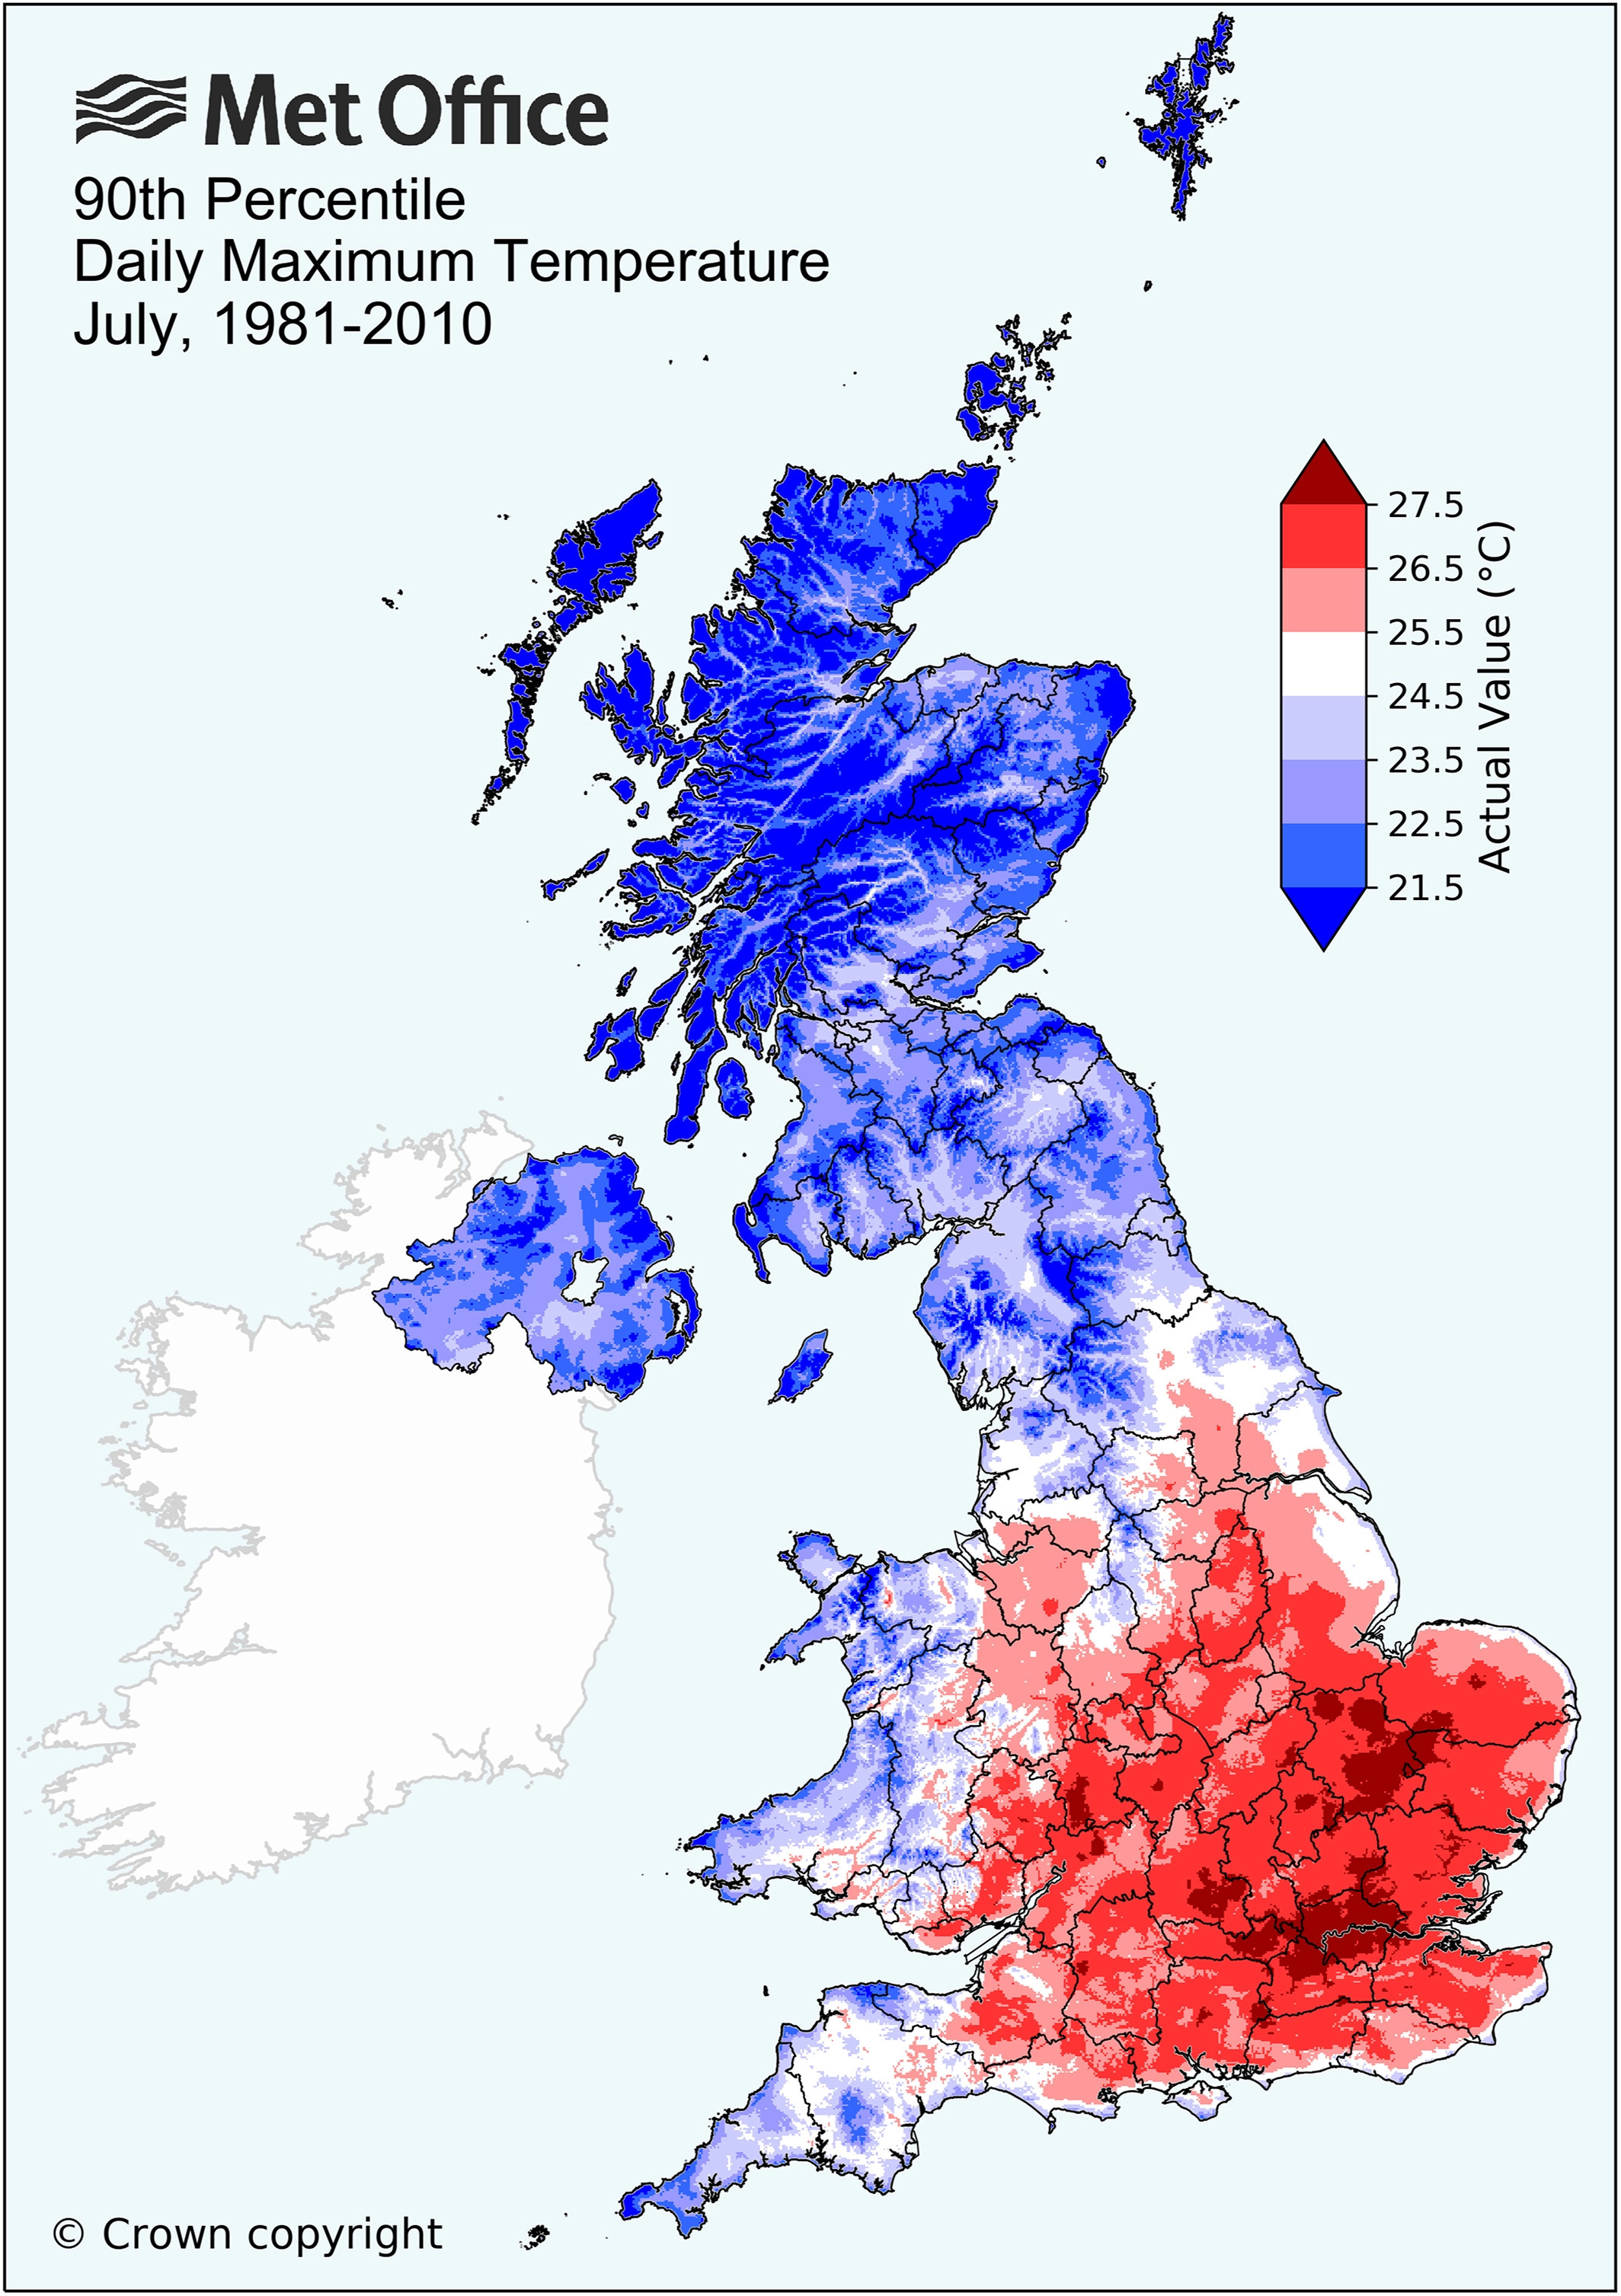
\includegraphics[width=\linewidth]{./mccarthy2019-fig3.jpg}
    \end{center}
    \caption{
    {\bf Plot from McCarthy \textit{et al.}, 2019.}
    \textit{The 90th percentile of July daily maximum temperatures (°C) determined on a 1 × 1km grid. England, Wales and Scotland county geographies are overlain.}\cite{McCarthy2019}
    }
    \label{McCarthy-fig3}
% \end{adjustwidth}
\end{figure}


\pagebreak

\section*{Materials and methods}

\subsection*{UKCP18 Data}
UKCP18 data consists of global, regional and local climate prediction data. 
For this project data from the land convection permitting model (CPM), HadREM3-RA11M, representing the relative concentration pathway (RCP) 8.5, was used with a spatial resolution of 2.2 km (local scale).
This model output consisted of 12 model runs (ensemble members) and a spatial average for the Greater London area was taken to ease computation.
The HadREM3-RA11M model was driven at it's boundary by perturbed variants of the Met Office Unified Model Global Atmosphere GA7 model (HadREM3-GA705) at 12km resolution, which in turn were driven by perturbed variants of the global HadGEM3-GC3.05 climate model at 60km resolution.\cite{UKCP18}

\noindent
The following meteorological variables were used in this project:
\begin{itemize}
    \item Maximum daily air temperature at 1.5m altitude (\texttt{tasmax})
    \item Daily mean relative humidity (\texttt{hurs})
    \item Daily mean surface wind speed (\texttt{sfcWind})
\end{itemize}
Data was downloaded from the Centre for Environmental Data Analysis (CEDA) archive via File Transfer Protocol (FTP).\cite{UKCP18data}

\subsection*{UTCI calculation}
For the purposes of this project the open source Python package PyMeteoSalute was used to calculate UTCI with precalculated polymonial coefficients.\cite{pymeteosalute}
UTCI values were calculated using \texttt{tasmax}, \texttt{hurs} and \texttt{sfcWind} from UKCP data.
$T_{mrt}$ was set to equal \texttt{tasmax}.
This was because $T_{mrt}$ cannot be calculated from the variables available in UKPC data.
This assumption is reasonable given that the UTCI reference conditions also set $T_{mrt}=T_a$, therefore allowing us to determine the effects of the $RH$ and $v_w$ on modulating $T_a$.


\subsection*{Heatwave analysis}
For the purposes of this project a heatwave is defined as three or more consecutive days above a given temperature threshold.
The thresholds used were 28°C, defined by the Met Office as the threshold for London\cite{McCarthy2019}, and 26°C, the temperature at which moderate heat stress is induced in UTCI theory.\cite{Blazejczyk2013}
\texttt{tasmax} data was compared against the 28°C, and calculated UTCI data was compared against both 28°C and 26°C thresholds.
The results were grouped by year so as to provide the annual number of hot days and heatwave events.

Box plots were made of the absolute number of days per year exceeding the threshold and the number of days per year within a heatwave event. 
These were grouped by decade.
Histograms were made for the number occurrences of consecutive hot days (i.e. heatwaves) of a certain length.
Given the low heatwave event frequency a logarithmic scale was used on the y-axes.
Poisson regressions were fitted to the histograms in order to understand the overall probability of long heatwaves for each decade.


All processing was conducted using the Python processing language.
Statistics and consecutive days analysis were calculated using the packages NumPy, Iris, Xarray and Pandas.
Plots were made using Matplotlib.











% Results and Discussion can be combined.
\section*{Results}



Plots
- Decadal box plots
- Poisson fits
- Report poisson lambdas

Results:
- Compare tasmax, utci and utci10
- 

\section*{Discussion}

Implications:
- UTCI with met office threshold not good
- UTCI does pick out heatwaves, but less than plain air temperature

Ways to improve:
- Tmrt excluded from UTCI calculation because not enough data to calculate it
    - Assumed Ta=Tmrt, but this is a substantial assumption i.e. air in thermal equilibrium with surroundings
    - Will exclude urban heat island effects, which are substantial [cit]
    - To what extent is urban heat island already accounted for in UKCP air temperature data?
    - Tmrt can't be applied to UTCI retroactively (e.g. once Exposure has been calculated) since UTCI relies on a 6th order polynomial calculation including every iteration of using Tmrt
    - \cite{Weihs2018}
- Humidity and windspeed used in UTCI calculation are daily means so not at same time of day as tasmax
    - However they don't affect the temperature strongly, so source of error is minimal
    - Tmrt is source of bigger error since effect is larger
    - Covariance matrices?
- 

Future exploration:
- Explore change in higher tiers of heat stress from UTCI data
- Tasmin (nighttime) temperatures ("tropical nights")
- Use incident radiation and cloud cover to improve UTCI calculation
- Use urban data to better model mean radiant temperature
- Use zero-inflated Poisson to fit heatwave duration graphs


\section*{Conclusion}




\cite{Askew2020}






\pagebreak

\bibliographystyle{plos2015}

\bibliography{CLIMAR-2021_Mar_report.bib}






% %%%%%%%%%%%%%%%%%%%%%%%%%%%%%%%%%%%%%%%%%%%%%%%%%%%%%%%%%%%%%%%%%%%%%%%%%%%%%%%%%%%%%%%%%%
% %%%%%%%%%%%%%%%%%%%%%%%%%%%%%%%%%%%%%%%%%%%%%%%%%%%%%%%%%%%%%%%%%%%%%%%%%%%%%%%%%%%%%%%%%%
% %%%%%%%%%%%%%%%%%%%%%%%%%%%%%%%%%%%%%%%%%%%%%%%%%%%%%%%%%%%%%%%%%%%%%%%%%%%%%%%%%%%%%%%%%%
% %%%%%%%%%%%%%%%%%%%%%%%%%%%%%%%%%%%%%%%%%%%%%%%%%%%%%%%%%%%%%%%%%%%%%%%%%%%%%%%%%%%%%%%%%%
% %%%%%%%%%%%%%%%%%%%%%%%%%%%%%%%%%%%%%%%%%%%%%%%%%%%%%%%%%%%%%%%%%%%%%%%%%%%%%%%%%%%%%%%%%%
\pagebreak
\section*{Supporting information}
% Include only the SI item label in the paragraph heading. Use the \nameref{label} command to cite SI items in the text.
\paragraph*{S1 Fig.}
\label{S1_Fig}
{\bf Bold the title sentence.} Add descriptive text after the title of the item (optional).



\subsection*{Subsection - Other sturff}



CO\textsubscript{2}


Eq~\ref{eq:schemeP}


Fig~\ref{fig1}


Table~\ref{table1} 


Citation~\cite{LaGennusa2005}




% Use "Eq" instead of "Equation" for equation citations.
\begin{eqnarray}
\label{eq:schemeP}
	\mathrm{P_Y} = \underbrace{H(Y_n) - H(Y_n|\mathbf{V}^{Y}_{n})}_{S_Y} + \underbrace{H(Y_n|\mathbf{V}^{Y}_{n})- H(Y_n|\mathbf{V}^{X,Y}_{n})}_{T_{X\rightarrow Y}},
\end{eqnarray}


% For figure citations, please use "Fig" instead of "Figure".
% Place figure captions after the first paragraph in which they are cited.
\begin{figure}[!h]
\caption{{\bf Bold the figure title.}
Figure caption text here, please use this space for the figure panel descriptions instead of using subfigure commands. A: Lorem ipsum dolor sit amet. B: Consectetur adipiscing elit.}
\label{fig1}
\end{figure}
to


\begin{itemize}
	\item First bulleted item.
	\item Second bulleted item.
	\item Third bulleted item.
\end{itemize}

% Place tables after the first paragraph in which they are cited.
\begin{table}[!ht]
\begin{adjustwidth}{-2.25in}{0in} % Comment out/remove adjustwidth environment if table fits in text column.
\centering
\caption{
{\bf Table caption Nulla mi mi, venenatis sed ipsum varius, volutpat euismod diam.}}
\begin{tabular}{|l+l|l|l|l|l|l|l|}
\hline
\multicolumn{4}{|l|}{\bf Heading1} & \multicolumn{4}{|l|}{\bf Heading2}\\ \thickhline
$cell1 row1$ & cell2 row 1 & cell3 row 1 & cell4 row 1 & cell5 row 1 & cell6 row 1 & cell7 row 1 & cell8 row 1\\ \hline
$cell1 row2$ & cell2 row 2 & cell3 row 2 & cell4 row 2 & cell5 row 2 & cell6 row 2 & cell7 row 2 & cell8 row 2\\ \hline
$cell1 row3$ & cell2 row 3 & cell3 row 3 & cell4 row 3 & cell5 row 3 & cell6 row 3 & cell7 row 3 & cell8 row 3\\ \hline
\end{tabular}
\begin{flushleft} Table notes Phasellus venenatis, tortor nec vestibulum mattis, massa tortor interdum felis, nec pellentesque metus tortor nec nisl. Ut ornare mauris tellus, vel dapibus arcu suscipit sed.
\end{flushleft}
\label{table1}
\end{adjustwidth}
\end{table}





\pagebreak


\begin{figure}
\begin{adjustwidth}{-2.25in}{0in}
    \begin{center}
        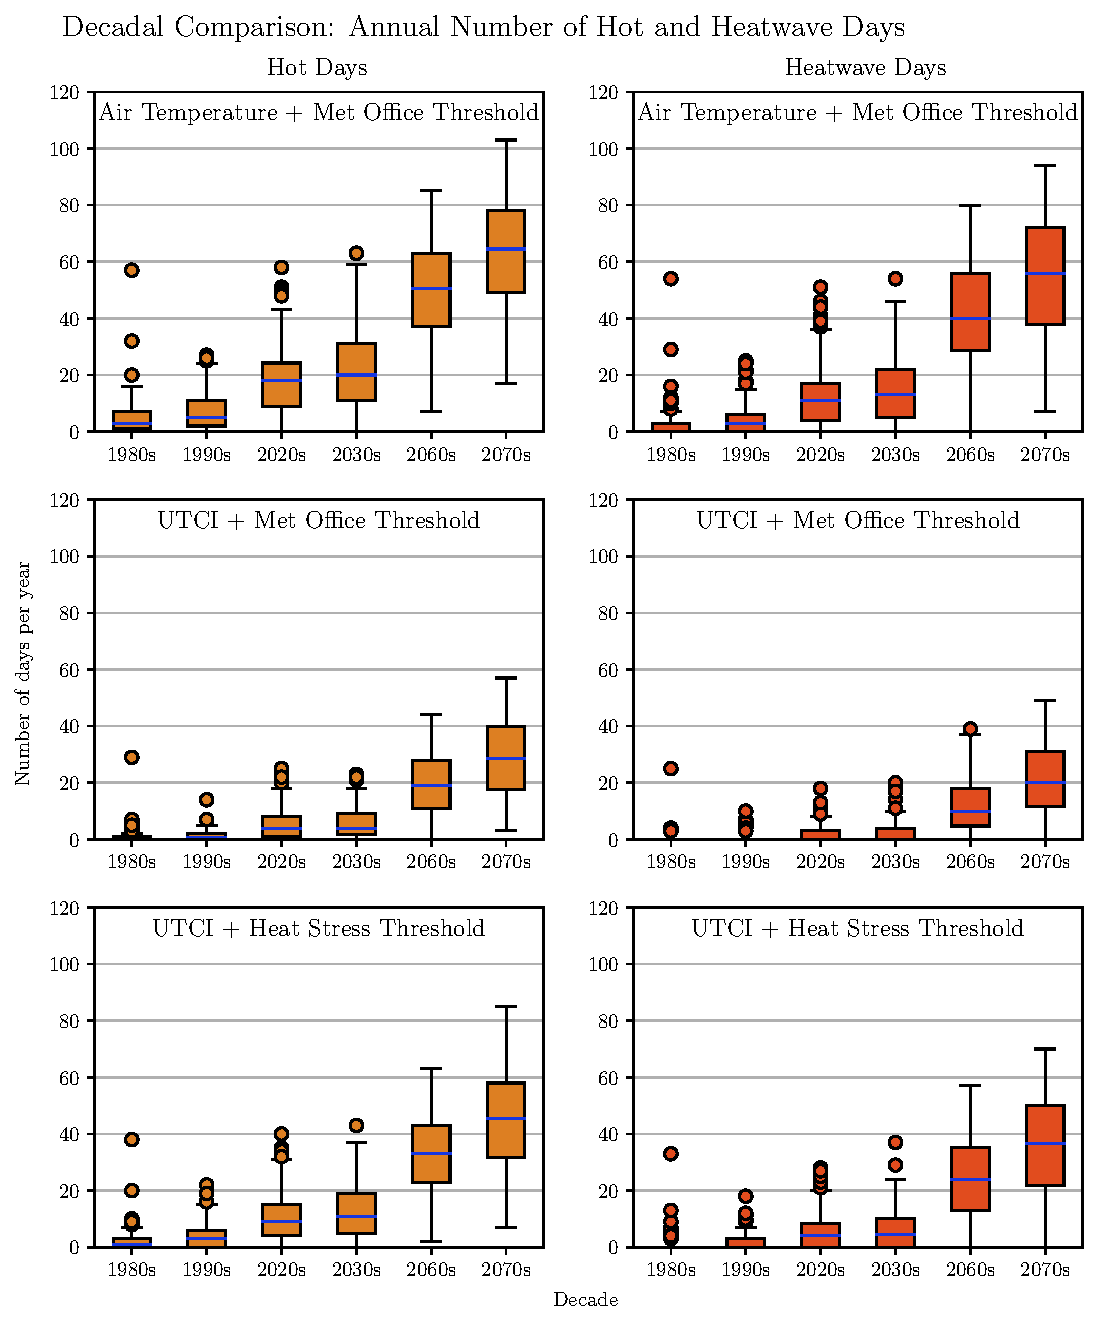
\includegraphics[width=0.9\linewidth]{./boxplots.pdf}
    \end{center}
    \caption{
    {\bf Annual number of hot and heatwave days increases over the decades modelled.}
    An accelerated increase is observed in the later decades of the 21\textsuperscript{st} century.
    Here hot days are defined as the total number of days in the year that exceed a threshold, whereas heatwave days are the total number of days in the year that are part of a continuous 3+ day heatwave. This analysis was done with raw and UTCI adjusted maximum daily air temperatures using thresholds defined by the Met Office and UTCI heat stress theory. Air temperature values for Greater London area used.
    }
    \label{boxplots}
\end{adjustwidth}
\end{figure}

\begin{figure}
\begin{adjustwidth}{-2.25in}{0in}
    \begin{center}
        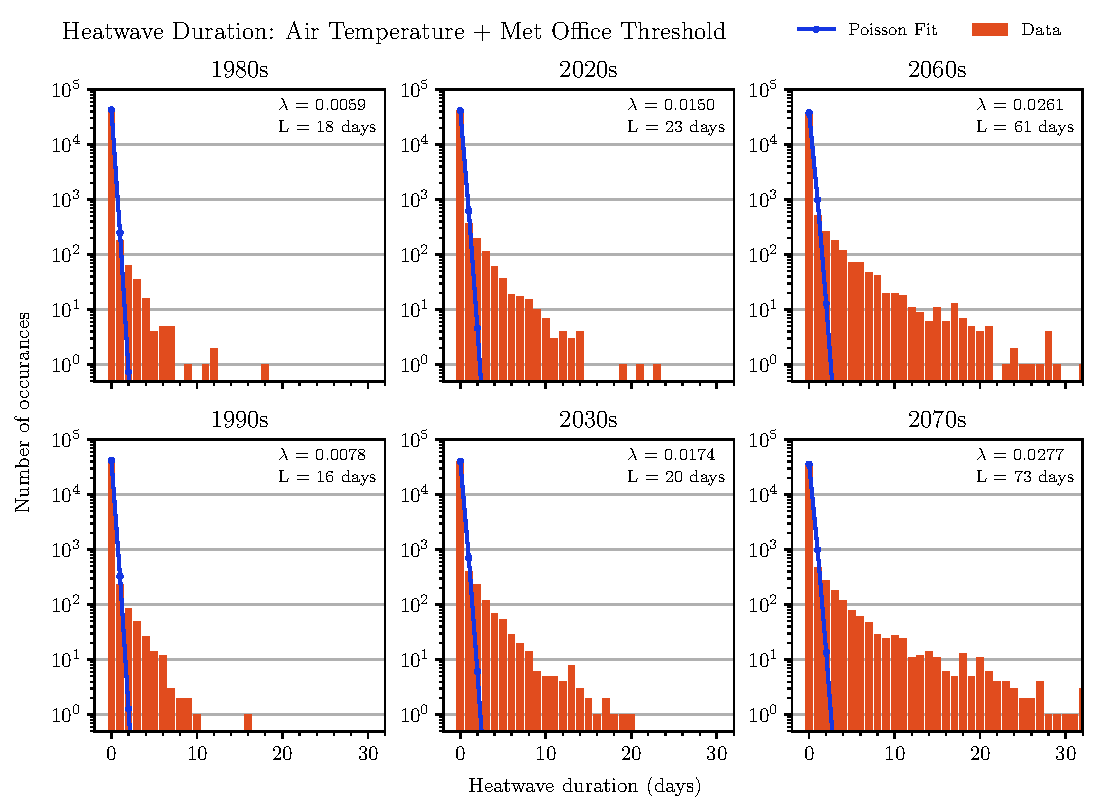
\includegraphics[width=\linewidth]{./tas_poisson.pdf}
    \end{center}
    \caption{
    {\bf Met Office heatwave definition predicts heatwaves up to 73 days long in the 2070s.}
    Comparison of all heatwave events across all years and ensemble members, grouped by decade.
    Here heatwave event duration is defined as a number of consecutive days in which the maximum daily air temperature exceeds the local climatologically defined threshold.
    Each decade has had a Poisson distribution fitted to it, with the resulting rate presented as $\lambda$.
    The longest contiguous heatwave in each decade is presented as $L$.
    Occurrence frequency is shown on a logarithmic scale so as to highlight low likelihood, high duration heatwave events.
    }
    \label{tas-poisson}
\end{adjustwidth}
\end{figure}

\begin{figure}
\begin{adjustwidth}{-2.25in}{0in}
    \begin{center}
        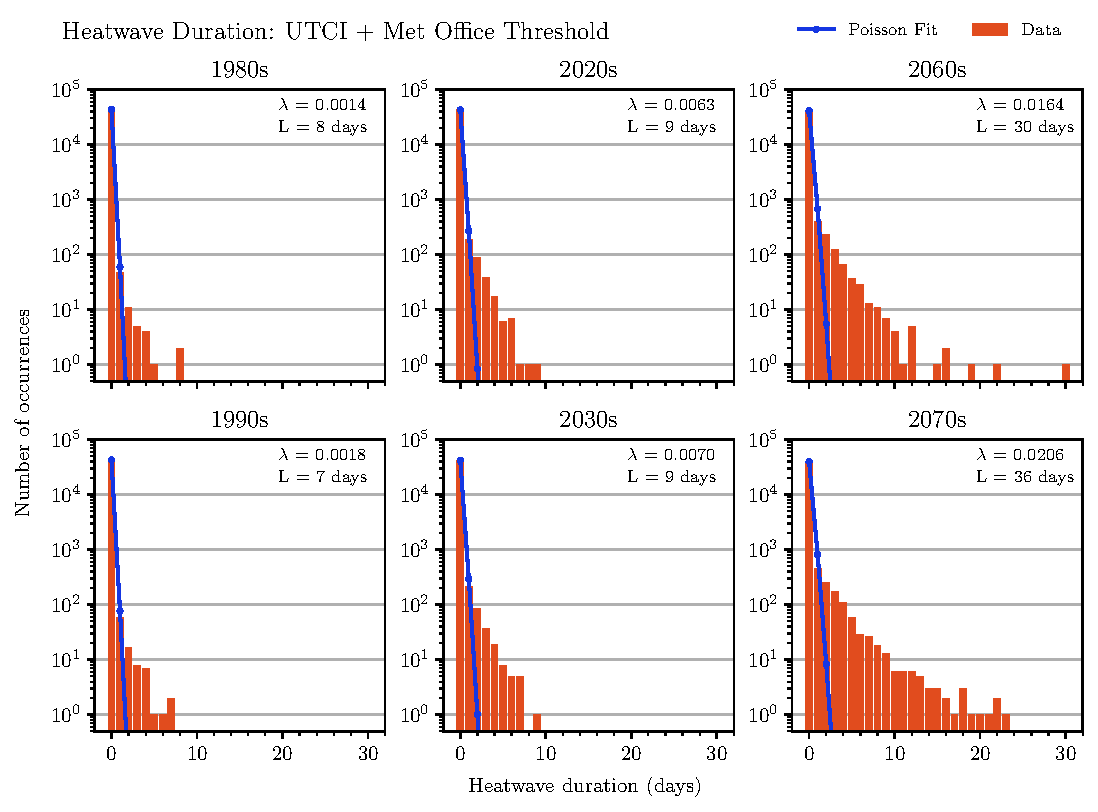
\includegraphics[width=\linewidth]{./utci_poisson.pdf}
    \end{center}
    \caption{
    {\bf UTCI with Met Office heatwave threshold predicts heatwaves up to 36 days long in the 2070s.}
    Comparison of all heatwave events across all years and ensemble members, grouped by decade.
    Here heatwave event duration is defined as a number of consecutive days in which the UTCI adjusted maximum daily air temperature exceeds the local climatologically defined threshold.
    Each decade has had a Poisson distribution fitted to it, with the resulting rate presented as $\lambda$.
    The longest contiguous heatwave in each decade is presented as $L$.
    Occurrence frequency is shown on a logarithmic scale so as to highlight low likelihood, high duration heatwave events.
    }
    \label{utci-poisson}
\end{adjustwidth}
\end{figure}

\begin{figure}
\begin{adjustwidth}{-2.25in}{0in}
    \begin{center}
        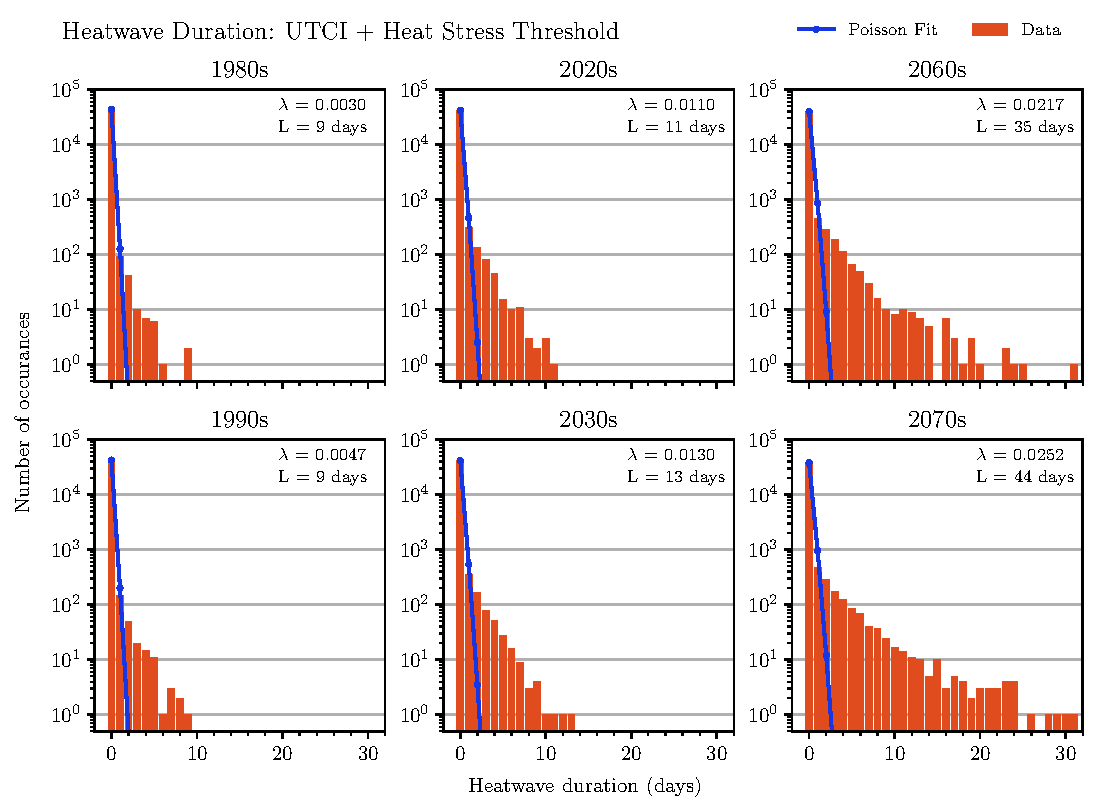
\includegraphics[width=\linewidth]{./u10_poisson.pdf}
    \end{center}
    \caption{
    {\bf UTCI heat stress definition predicts heatwaves up to 44 days long in the 2070s.}
    Comparison of all heatwave events across all years and ensemble members, grouped by decade.
    Here heatwave event duration is defined as a number of consecutive days in which the UTCI adjusted maximum daily air temperature exceeds the UTCI theoretical heat stress threshold.
    Each decade has had a Poisson distribution fitted to it, with the resulting rate presented as $\lambda$.
    The longest contiguous heatwave in each decade is presented as $L$.
    Occurrence frequency is shown on a logarithmic scale so as to highlight low likelihood, high duration heatwave events.
    }
    \label{u10-poisson}
\end{adjustwidth}
\end{figure}







\end{document}

